\documentclass{article}
\usepackage[utf8]{inputenc}
\usepackage{titling}
\usepackage{graphicx}
\usepackage{xcolor}
\usepackage[colorlinks=true,linkcolor=darkgray]{hyperref}
\usepackage[spanish]{babel}


\title{Práctica 3.1: Servidor DNS Maestro sin chroot}
\author{Cristina Díaz García}
\date{Noviembre 2018}

\renewcommand\maketitlehooka{\null\mbox{}\vfill}
\renewcommand\maketitlehookd{\vfill\null}


\begin{document}

\addcontentsline{toc}{section}{Índice general}

\begin{titlingpage}
\maketitle
\end{titlingpage}

\newpage

\tableofcontents

\newpage

\section{Modificación de \textit{/etc/bind/named.conf.local}}

\begin{center}
	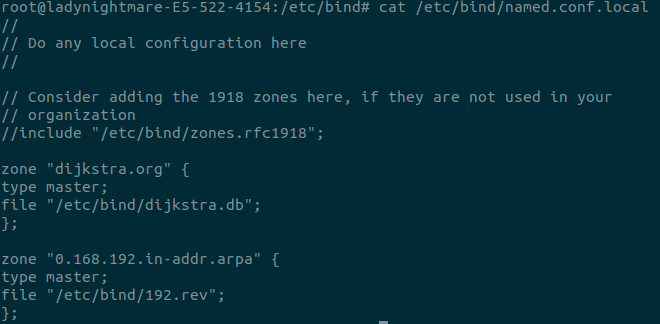
\includegraphics[scale=0.5]{PoniendoZonas.png} 
\end{center}

\section{Archivo de zona de búsqueda directa (.db)}

\begin{center}
	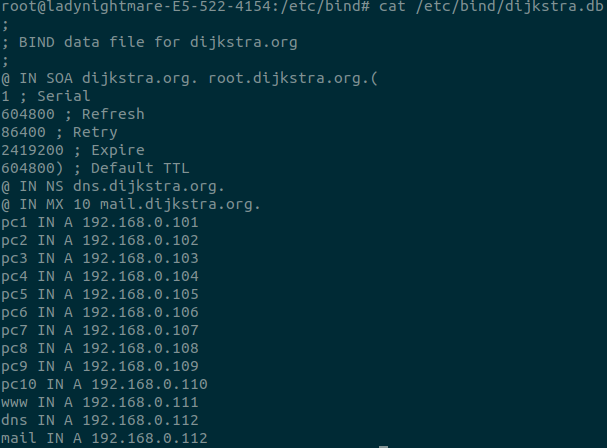
\includegraphics[scale=0.5]{db.png} 
\end{center}

\section{Archivo de zona de búsqueda inversa}

\begin{center}
	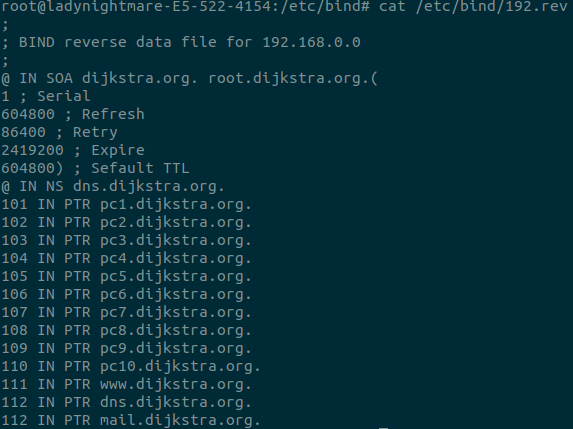
\includegraphics[scale=0.5]{inv.png} 
\end{center}

\section{Configuración de servidor DNS}

\begin{center}
	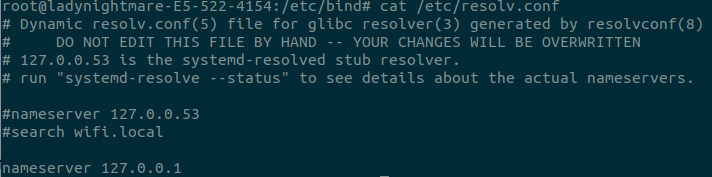
\includegraphics[scale=0.5]{resolv.png} 
\end{center}

\section{Uso de la DNS}

\subsection{Inicialización de la DNS}

\begin{center}
	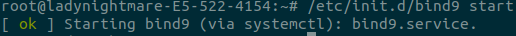
\includegraphics[scale=0.5]{start.png} 
\end{center}

\subsection{Comprobación del estado de la DNS}

\begin{center}
	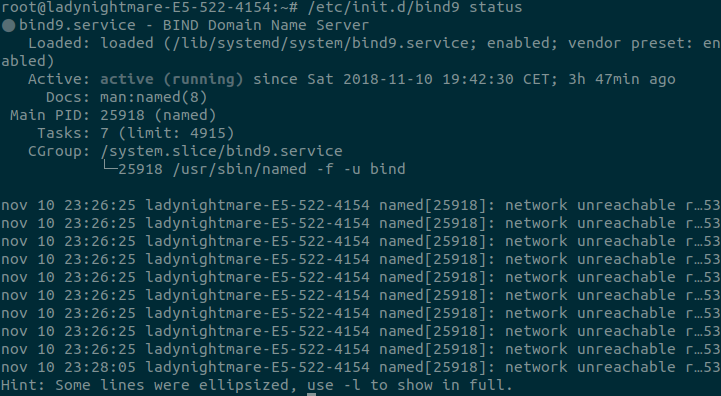
\includegraphics[scale=0.5]{status.png} 
\end{center}

\subsection{Resolución de peticiones}

\begin{center}
	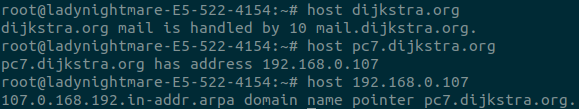
\includegraphics[scale=0.5]{hosts.png} 
\end{center}

\subsection{Apagado de la DNS}

\begin{center}
	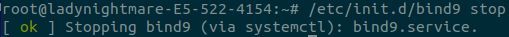
\includegraphics[scale=0.5]{stop.png} 
\end{center}

\subsection{Comprobación del estado de la DNS}

\begin{center}
	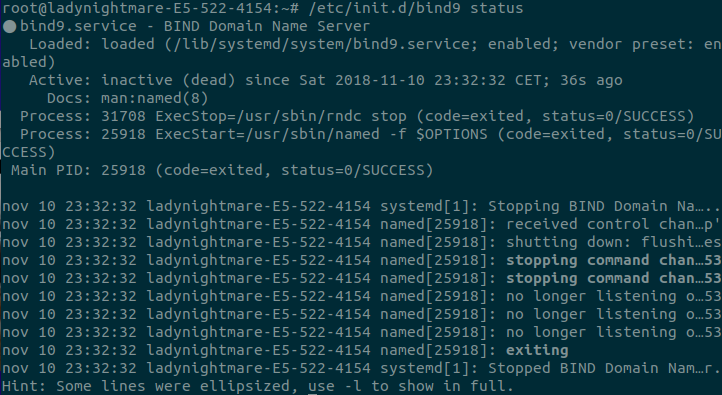
\includegraphics[scale=0.5]{status2.png} 
\end{center}

\end{document}